\documentclass[10pt]{article}
\setlength{\textwidth}{6.3in}
\setlength{\textheight}{9in}
\setlength{\oddsidemargin}{0in}
\setlength{\evensidemargin}{0in}
\setlength{\topmargin}{-.5in}
%\parindent=0in
\linespread{1.3}
\usepackage{ mathrsfs }
\usepackage{amsthm}
\usepackage{ amssymb }
\usepackage{graphicx}
\newtheorem{theorem}{Theorem}[section]
\newtheorem{lemma}[theorem]{Lemma}

\usepackage{amsmath}
\usepackage{amsfonts}
\usepackage{fancyhdr}
\pagestyle{fancy}
\headheight = 14.5pt
\lhead{Probability HW6, Thomas Zeng }
\rhead{Math 240, Fall 2022}
\cfoot{\thepage}

\begin{document}
\section*{1}
\subsection*{a}

\begin{align*}
    E[X] &= m'(0)\\
    &= \left(\frac{1}{pe^t}-\frac{1-p}{p}\right)^{-1}\frac{d}{dt}\Bigr |_0\\
    &= -\left(\frac{1}{pe^t}-\frac{1-p}{p}\right)^{-2}\left(-\frac{1}{pe^t} \right)\Bigr |_0\\
    &= -\left(\frac{1}{p}-\frac{1-p}{p}\right)^{-2}\left(-\frac{1}{p}\right)\\
    &= 1^{-2}\frac{1}{p}\\
    &= \frac{1}{p}
\end{align*}

\subsection*{b}

\begin{align*}
    E[X] &= m'(0)\\
    &=e^{5t+t^2}\frac{d}{dt}\Bigr |_0\\
    &=e^{5t+t^2}(5+2t)\Bigr |_0\\
    &=5
\end{align*}

\subsection*{c}

\begin{align*}
    E[X^2] &= m''(0)\\
    &= e^{5t+t^2}(5+2t)\frac{d}{dt}\Bigr |_0 \quad \text{first deriv. calculated above}\\
    &= e^{5t+t^2}(5+2t)^2 + e^{5t+t^2}2\Bigr |_0\\
    &= 25+2\\
    &= 27
\end{align*}

\begin{align*}
    V[X] &= E[X^2] - E[X]^2\\
    &= 27 - 5^2\\
    &= 2
\end{align*}

\section*{2}
Let us define $m_X$ as mgf of $X$ and $m_{X_i}$ as mgf for each $X_i.$
\begin{align*}
    m_X(t) &= \prod_{i=1}^nm_{X_i}(t)\\
    &= (1-p+pe^t)^n
\end{align*}

\section*{3}
Let us define $m_X$ as mgf of $X$ and $m_Y$ as mgf of $Y$ and $m_W$ as mgf of $W.$

\begin{align*}
    m_W(t) &= m_Y(2t)m_X(t)\\
    &=e^{\lambda(e^{2t}-1)}e^{\lambda(e^t-1)}\\
    &=e^{\lambda(e^{2t}-1) + \lambda(e^t-1)}\\
    &=e^{\lambda(e^{2t}-1+e^t-1)}\\
    &=e^{\lambda(e^t(e^t+1)-2)}
\end{align*}
This is not Poisson.

\section*{4}

Let us define $X \sim \text{Hypergeom}(20,100, 15).$ Our lake follows this distribution as we have $r=20$ tagged fish, $N=100$ total fish in the lake and $n=15$ sampled fish.

To compute the probability of $k$ tagged fish, it would thus be $\frac{\binom{20}{k}\binom{80}{15-k}}{\binom{100}{15}}$. For $k=4$ we thus have
\[ \frac{\binom{20}{4}\binom{80}{11}}{\binom{100}{15}}\approx0.20.\]

\section*{5}
\subsection*{a}
$X\sim\text{Binom}(5,0.1)$
\subsection*{b}
$X\sim\text{Geom}(0.1)$
\subsection*{c}
$X\sim\text{Nbinom}(5, 0.1)$
\subsection*{d}
We want $Pr(X\le20)$ which is approx $0.043$ using R command \texttt{pnbinom(20-5,5,.1)}.

\section*{6}
\subsection*{a}
$X\sim\text{Geom}(0.001)$
\subsection*{b}
$\frac{1}{p}=\frac{1}{0.001}=1000.$
\subsection*{c}
$1000-1=999.$
\subsection*{d}
$P(X>1000)=(1-0.001)^{1000}\approx0.368$
\subsection*{e}
$Y\sim\text{Nbinom}(3, 0.01)$
\subsection*{f}
$\frac{r}{p}=\frac{3}{0.001}=300$
\subsection*{g}
$\sigma(X) = V(X)^{0.5} = \sqrt{\frac{1-p}{p^2}} = \sqrt{\frac{1-0.001}{0.01^2}}\approx 9.995$

\noindent
$\sigma(Y) = V(Y)^{0.5} = \sqrt{\frac{r(1-p)}{p^2}}= \sqrt{\frac{3(1-0.001)}{0.01^2}}\approx17.3$

It makes sense that there is more variability in $Y$ than $X$ as in $Y$ we are looking for more defective phones ($3$ vs $1$). Hence, there are more combinations of ways to select phones before finding $3$ defective phones than $1$ -- hence the greater variability.

\section*{7}
%5.20
\subsection*{a}
We use \texttt{dnbinom(6-3,3,.4)} which gives us $0.13824.$
\subsection*{b}
We use \texttt{pnbinom(10-3,3,.4)-pnbinom(4-3,3,.4)} which gives us $0.654.$
\subsection*{c}
We use \texttt{1-pnbinom(7-3,3,.4)} which gives us $0.420.$

\section*{8}
%5.46
The probability of choosing a prime number is $\frac{10}{30}=\frac{1}{3}.$ Let $X$ be the number of days with no homework, then $X\sim\text{Binom}(42,\frac{1}{3}).$ $E[X]=np=\frac{42}{3}=14.$

\section*{9}
%5.48
Let $X$ be the number of winners Jenna got. Then $X\sim\text{Hypergeom}(6,30,10).$ We want $P(X=3)\approx0.23$ using $\texttt{dhyper(3,6,30-6,10)}.$

\section*{10}
\subsection*{a}
Using Mathematica:
    \begin{verbatim}
Plot[Piecewise[{{0, x < 0}, {1-E^(-x/3), x >= 0}}], {x, -2, 10}, PlotRange->{-0.1,1}]\end{verbatim}
we get a plot like the following.
\begin{center}
    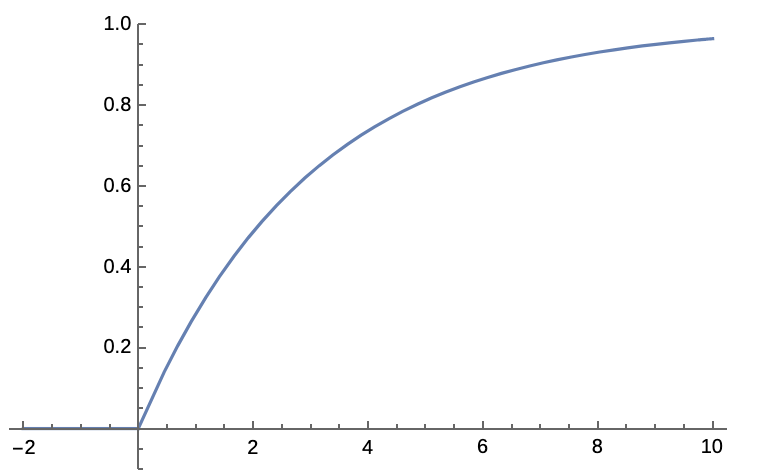
\includegraphics[width=0.5\textwidth]{hw6_10.png}
\end{center}
This satisfies CDF as it is non-decreasing, right continuous, and $F(-\infty)=0, F(\infty)=1.$
\subsection*{b}
$F(2)=1-e^{-2/3}\approx0.487.$
\subsection*{c}
$F(2)-F(1)=1-e^{-2/3}-(1-e^{-1/3})\approx0.203$
\subsection*{d}
For $x>0$ we have
\begin{align*}
    f(x) &= F(x)\frac{d}{dx}\\
    &= 1-e^{-x/3}\frac{d}{dx}\\
    &=\frac{1}{3}e^{-x/3}
\end{align*}
Thus in general, we have
\begin{equation*}
    f(x)=\begin{cases}
        \frac{1}{3}e^{-x/3},\; x>0\\
        0,\; \text{o.w.}
    \end{cases}
\end{equation*}
\end{document}